\subsubsection{Die Bibliothek \emph{gdata}}
Die Google-Bibliothek \emph{gdata} ist eine frei verf\"ugbare Bibliothek zum erstellen von
 Clientapplications für die Services der Google-Cloud.
\emph{gdata} kapselt die Webservices komplett in Java-Klassen, so dass ein importieren
 (z.\ B.\ mit \emph{wsimport}) nicht mehr notwendig ist.

In der Beschreibung der \emph{gdata}-Bibliothek wird beschrieben, wie man aus der zip-Datei
 ein JAR compilieren kann, da dies bei mir in mehreren Versuchen nicht geklappt hat,
 haben wir die pragmatische Lösung gewählt und die in der zip-Datei enthaltenen JARs von Hand
 in das Projekt eingefügt.
%TODO Link zu gdata

\subsubsection{Authentifizieren und Verbinden mit \emph{gdata}}
Google bietet zwei Authentifizierungsverfahren an
\begin{enumerate}
	\item\emph{OAuth}
	\item Username und Passwort
\end{enumerate}
\emph{OAuth} ist ein Service, der bei erfolgreicher Anmeldung ein Token erstellt, mit dem
 der Client von Google bereitgestellte Services aufrufen und sich authentifizieren kann.
So muss der Client die Anmelde-Daten des Nutzers nicht speichern, sondern nur den Token.
In Abbildung \ref{fig:google_oauth} wird ein Beispiel f\"ur die Nutzung von \emph{OAuth} dargestellt.
\begin{figure}[h!]
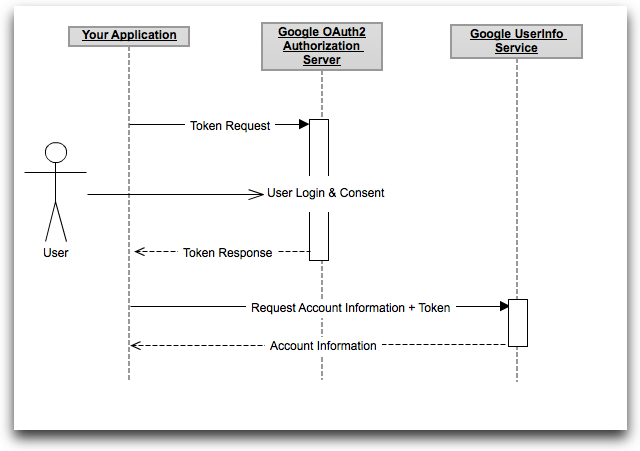
\includegraphics[width=\textwidth]{Bilder/googleOauth.png}
\caption{Nutzungsbeispiel f\"ur \emph{OAuth}\cite{GO01}}
\label{fig:google_oauth}
\end{figure}

Da wir unseren eigenen Account nutzen und die Daten nicht sicherheitskritisch sind, haben
 wir die zweite Variante gew\"ahlt und authentifizieren uns bei jedem Service-Aufruf mit
 Username und Passwort.

Die Authentifizierung wird für ein \emph{ContacsService}-Objekt, wie in Listing
 \ref{lst:authpwbeispiel} abgebildet, einmal durchgeführt, danach wird sie vom Framework
 automatisch durchgeführt.

\javalstset{Beispiel für die Authentifizierung ohne \emph{OAuth}}{lst:authpwbeispiel}
\begin{lstlisting}
ContactsService myService;
myService = new ContactsService(servicename);
try {
	myService.setUserCredentials(username, password);
} catch (AuthenticationException e) {
	e.printStackTrace();
}
\end{lstlisting}

\subsubsection{Kontakte suchen}
Die \emph{gdata}-Bibliothek bietet die Möglichkeit, Kontakte wie in Listing \ref{lst:searchQuery}
 mit Angabe eines \emph{Querys} herunterzuladen.
Das \emph{Query} kann jedoch nur zwischen Gruppen unterscheiden, jedoch nicht nach anderen
 Kriterien wie z.\ B.\ dem Vornamen oder dem Nachnamen eines Kontakts filtern.

\javalstset{Kontaktsuche per Query}{lst:searchQuery}
\begin{lstlisting}
URL feedUrl = new URL(contactsURL);
Query myQuery = new Query(feedUrl);
ContactFeed resultFeed = null;
// Gruppe
String groupId = null;
// Parameter Contact filter
switch (filter.getType()) {
case CUSTOMER:
	groupId = customerGroupURL;
	break;
case SUPPLIER:
	groupId = supplierGroupURL;
	break;
case EMPLOYEE:
	groupId = employeeGroupURL;
	break;
default:
	break;
}
myQuery.setStringCustomParameter("group", groupId);
// submit request
resultFeed = myService.getFeed(feedUrl, ContactFeed.class);
\end{lstlisting}

Das Suchen von Kontakten geschieht in unserem Projekt durch das Herunterladen aller Kontakte
 einer Gruppe und anschließendem sortieren "`von Hand"'.

\subsubsection{Kontakte einf\"ugen}
Das Einfügen von Kontakten ist über ein erstelltes Service-Objekt 

\javalstset{Kontakt-Objekt erstellen}{lst:createContact}
\begin{lstlisting}
// Create the entry to insert
ContactEntry contact = new ContactEntry();
contact.setTitle(new PlainTextConstruct(contactInfoCopy.getFirstname()
		+ contactInfoCopy.getLastname()));
\end{lstlisting}

\javalstset{Namen in ein Kontakt-Objekt einfügen}{lst:ccsetname}
\begin{lstlisting}
// Name
Name name = new Name();
name.setFamilyName(new FamilyName(contactInfoCopy.getLastname(), null));
name.setGivenName(new GivenName(contactInfoCopy.getFirstname(), null));
contact.setName(name);
\end{lstlisting}

\javalstset{Benutzerdefinierte Einträge zu einem Kontakt-Objekt hinzufügen}{lst:cccustomEntry}
\begin{lstlisting}	
// Firma
if (contactInfoCopy.getCompany() != null) {
	ExtendedProperty company = new ExtendedProperty();
	company.setName(DLI_GoogleContactsConnector.company);
	company.setValue(contactInfoCopy.getCompany());
	contact.addExtendedProperty(company);
}
\end{lstlisting}

\javalstset{Den Kontakt einer Gruppe hinzufügen}{lst:ccjoingroup}
\begin{lstlisting}
// Gruppe setzen
String groupURL = null;
switch (contactInfoCopy.getType()) {
case CUSTOMER:
groupURL = customerGroupURL;
contact.addGroupMembershipInfo(new GroupMembershipInfo(false, groupURL));
\end{lstlisting}

\javalstset{Das Kontakt-Objekt senden}{lst:ccsendcontact}
\begin{lstlisting}
// Kontakt senden		
URL postUrl = new URL(contactsURL);
return myService.insert(postUrl, contact);
\end{lstlisting}